\documentclass{article}
\usepackage{caption}
\usepackage{amssymb}
%\usepackage{array}
\usepackage{geometry}
%\usepackage{scrextend}
\usepackage{amsmath}
%\usepackage{hyperref}
\usepackage{graphicx}
\usepackage{pdfpages}
%\usepackage{multicol}
\usepackage{tabularx}
\usepackage{float}

\title{EE102 Homework 2}
\author{Jacob Guenther}

\geometry{
	a4paper,
	total={170mm,257mm},
	left=20mm,
	top=20mm,
}

\begin{document}

\includepdf[pages=1,pagecommand={}]{Lab_3_cover.pdf}

\section{Objective}
In this lab we learn how to compile and upload a program to an Arduino Nano using the Arduino IDE. We also gain experience using an oscilloscope by using it to measure frequency.

\section{Equipment}
\begin{itemize}
	\item Ocilloscope
	\item Arduino Nano
	\item Resistors
	\item Potentiometer
	\item LEDs
	\item Breadboard
	\item Jumpers
\end{itemize}

\section{Setup}

\paragraph{}
For the first experiment we use the schematic shown if figure (1). We probe the circuit with the occiliscope at digital pin 9 and ground.

\begin{figure}[H]
	\begin{center}
	\includegraphics[width=10cm]{schematic_led}
	\end{center}
	\caption{Schematic used to create a 25kHz frequency with a 30\% duty cycle.}
\end{figure}

\paragraph{}
In the second experiment we use the circuit shown if figure (2).

\begin{figure}[H]
	\begin{center}
	\includegraphics[width=11cm]{lab_3_schematic_4_led}
	\end{center}
	\caption{Schematic used to measure voltage on an analog input and display the value of that voltage using LEDs.}
\end{figure}

\section{Observations and Results}

\paragraph{}
We use the circuit shown in figure (1) along with the code shown in figure (3) to produce the plot shown in figure (4). The code was moddified so that the duty is 30\% instead of 50\%. To do this we multiply 1023 by 0.3. 1023 is the max value for the duty cycle.

\paragraph{}
From the plot we can see that the max voltage is 4.65 volts. The period between peaks is 39.8 us, and the frequency of the square wave is 25.126 kHz. The positioning of the reference lines may be slightly off.

\begin{figure}[H]
	\includegraphics[width=10cm]{code_part_1}
	\caption{Code for 25kHz frequency with 30\% duty cycle.}
\end{figure}

\paragraph{}
\begin{figure}[H]
	\begin{center}
	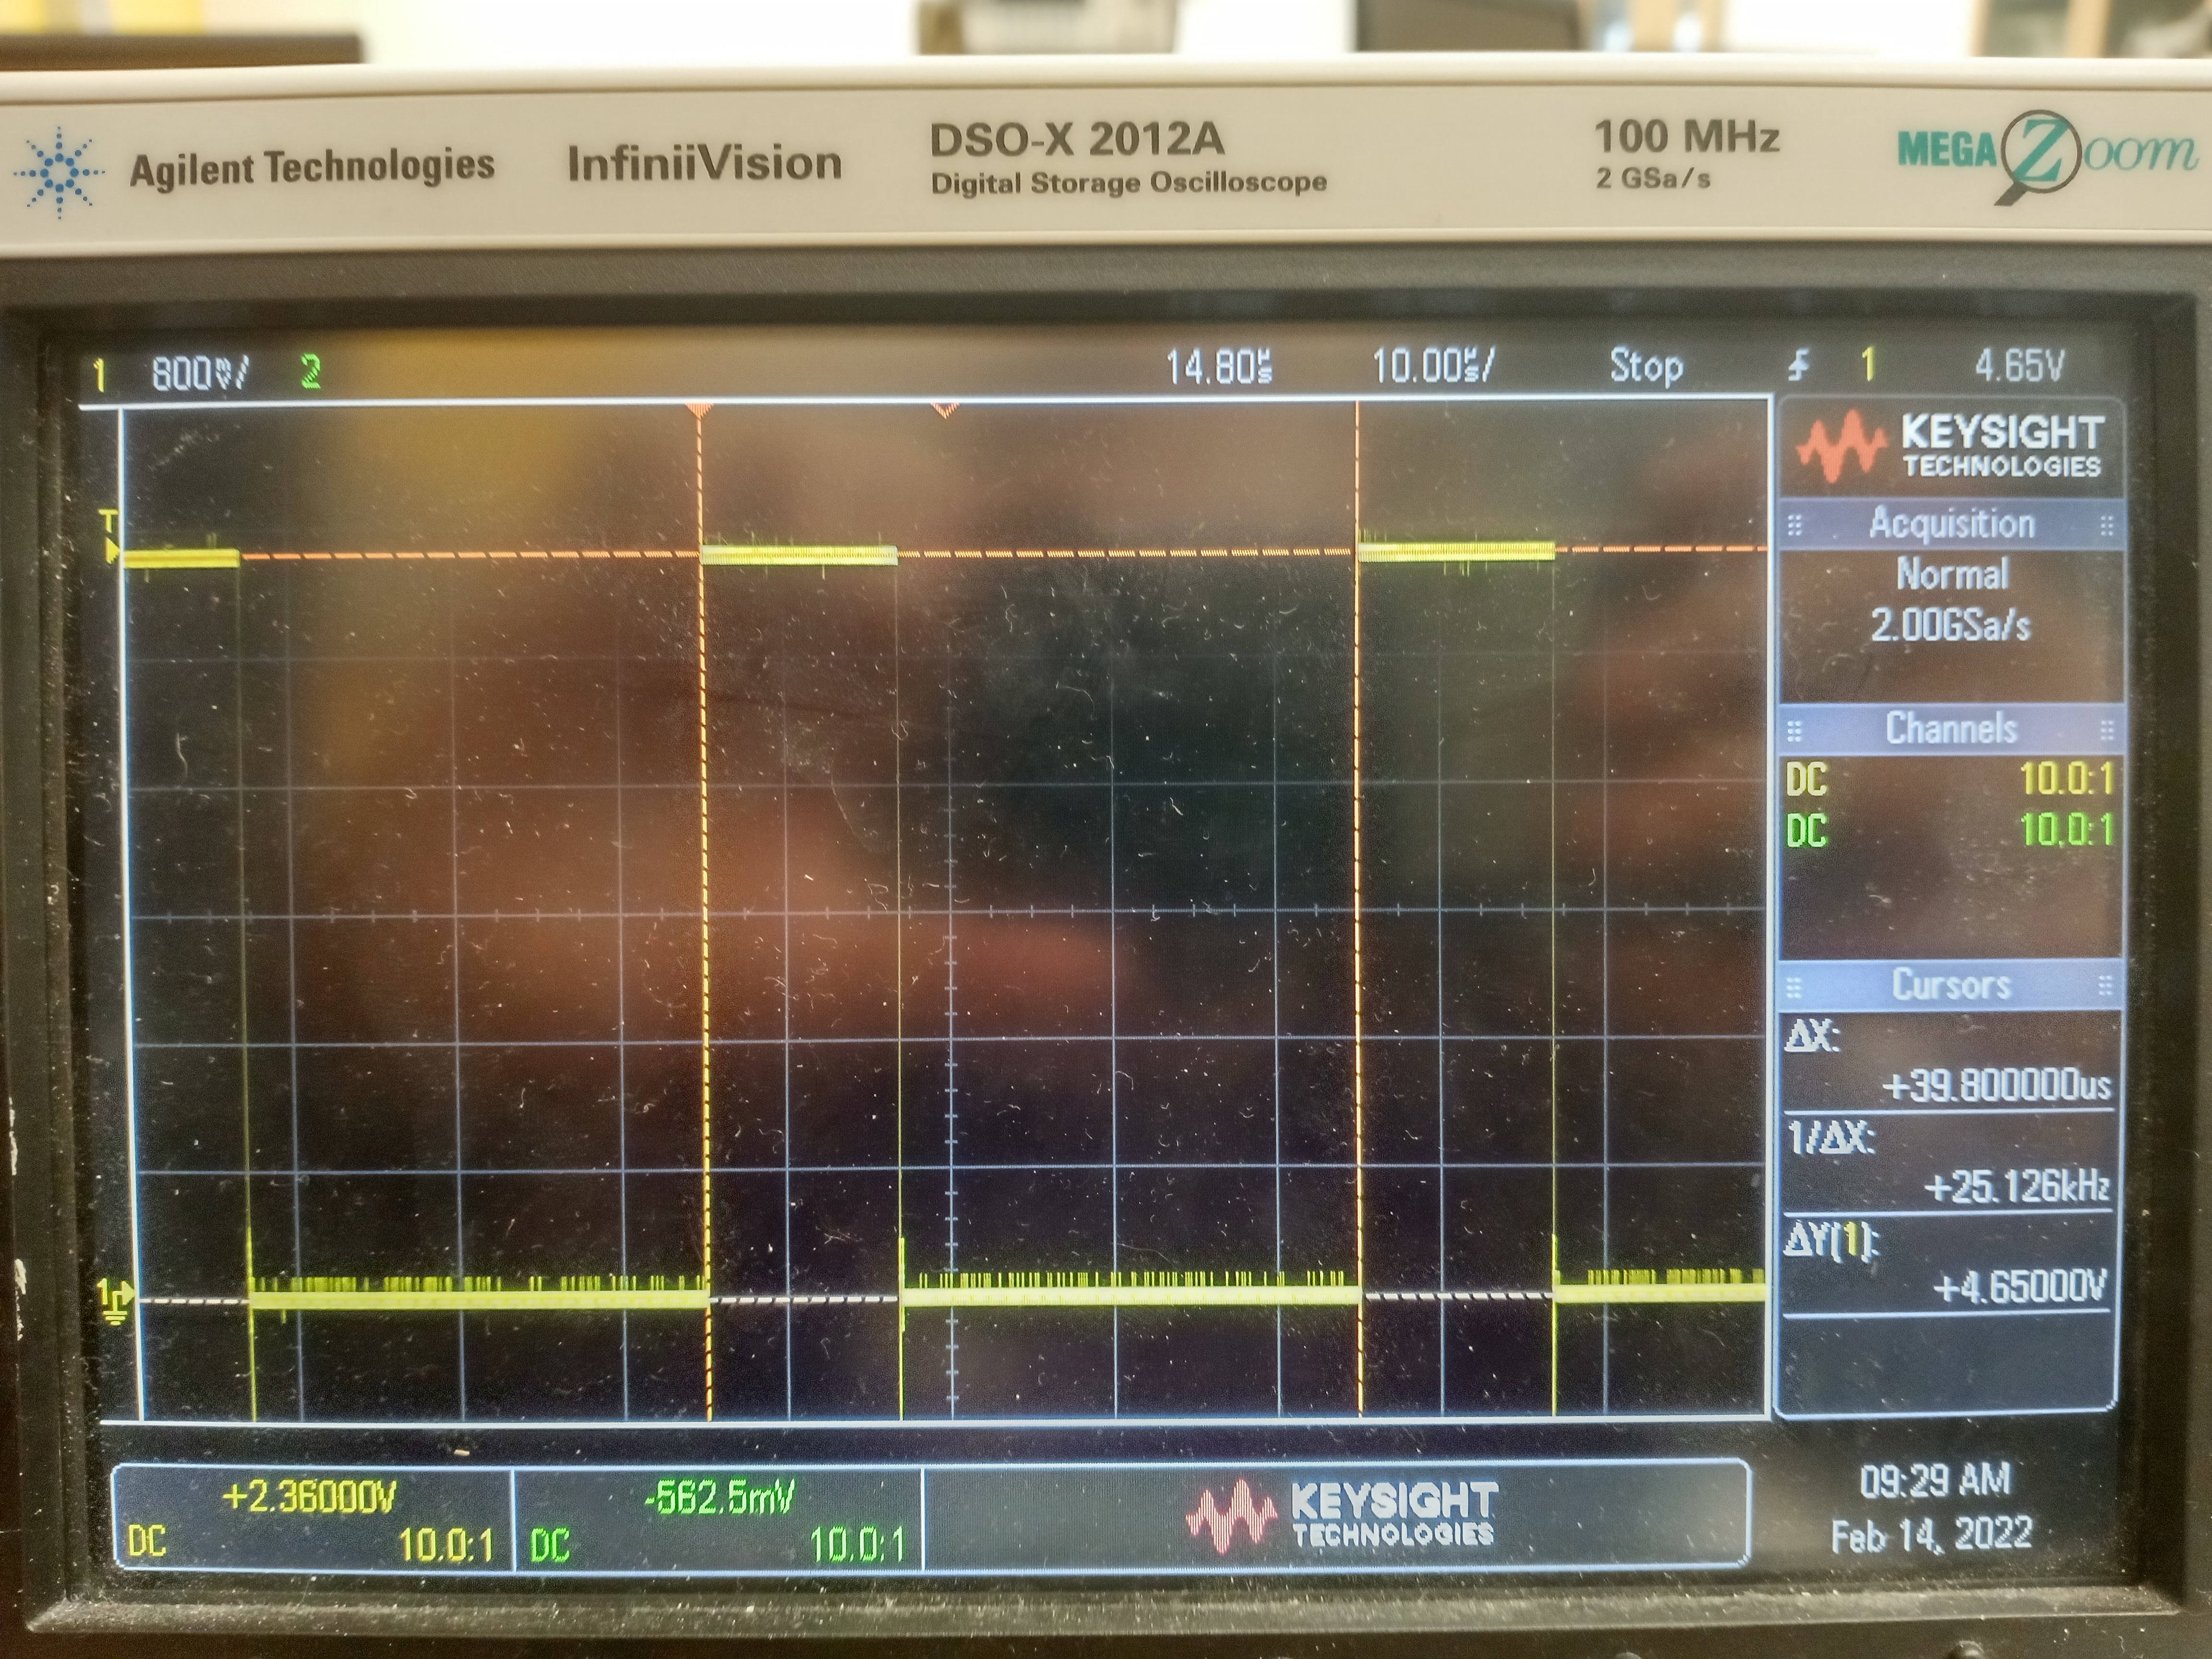
\includegraphics[width=12cm]{ocilliscope_plot}
	\end{center}
	\caption{The plot of the occiliscope showing a 25 kHz frequency with a 30\% duty cycle.}
\end{figure}

\paragraph{}
In the next part of the lab we use the circuit shown in figure (2) along with the code shown in figure (5) to indicate the voltage at anolog pin 0. The code was modified from the provided code by using else if statements to turn on only 1 LED.

\begin{figure}[H]
	\begin{center}
		\includegraphics[width=11cm]{code_part_2}
	\end{center}
	\caption{Code used to turn on an LED depending on the measured voltage at anolog pin 0.}
\end{figure}


\newpage
\section{Conclusion}
In this lab we learned how to program an Arduino using the Arduino IDE. We used the PWM functionality of some of the digital pins, to create a specific square wave. Finally we programmed the Arduino to read an analog input and display the voltage using a digital output pin.

\paragraph{}
To read a temperature using a thermistor we can use a voltage divider with the thermistor, resistor, and an anolog input pin. Then we can convert the analog value to voltage, and then convert to voltage to temperature.

\newpage
\section{References}
\noindent
[1] Denise Thorsen, Maher Al-Badri, INTRODUCTION TO ELECTRICAL AND COMPUTER ENGINEERING, University of Alaska Fairbanks, 2022.
\newline
\newline
\noindent

\end{document}